\section{The Neural Tactic and Difficulty Model}\label{sec:nn-results}

PuzzleNet was trained on the 5{,}526{,}626 puzzles of the training split for three epochs (8{,}097
updates of 2{,}048 puzzles), which took 42 minutes on the development laptop's CPU. The 59{,}668
puzzles of the held-out labeller harness were excluded from training and from model selection, so the
comparison below is on exactly the puzzles the rule-based tagger was scored on in
Section~\ref{sec:labeller-results}, with neither labeller having seen them.

\subsection{Tactic labelling}\label{sec:nn-labelling}

\begin{table}[H]
\centering
\small
\caption{Labeller agreement with Lichess themes on the held-out harness (seed 11). Uniform sample
$n = 30{,}000$; stratified sample $n = 48{,}000$. The rule-based row reproduces
Section~\ref{sec:labeller-results} exactly, which confirms that both labellers see the same
puzzles.}\label{tab:nn-harness}
\begin{tabularx}{\linewidth}{Xccccc}
\toprule
\textbf{Labeller} & \textbf{Strict} & \textbf{Lenient} & \textbf{$\kappa$} & \textbf{Macro recall} & \textbf{Macro precision} \\
\midrule
Rule-based tagger & 58.4\% & 60.9\% & 0.516 & 0.320 & 0.537 \\
\textbf{PuzzleNet} & \textbf{92.6\%} & \textbf{93.1\%} & \textbf{0.913} & \textbf{0.859} & \textbf{0.877} \\
\bottomrule
\end{tabularx}
\end{table}

\begin{finding}[The labeller stops being the bottleneck]
Agreement rises from 58.4\% to 92.6\% and $\kappa$ from 0.52 to 0.91, which moves the labeller from
``moderate'' to ``almost perfect'' on the Landis and Koch scale~\cite{landis1977measurement}. Because
both labellers ran on the same puzzles, the comparison is paired: PuzzleNet is right on 10{,}671
puzzles where the rules are wrong, and wrong on 424 where the rules are right (McNemar's exact test,
$p < 10^{-300}$). Bootstrap 95\% intervals for the differences are $+33.6$ to $+34.7$ points of
agreement, $+0.391$ to $+0.403$ of $\kappa$, and $+0.536$ to $+0.543$ of macro recall.
\end{finding}

\begin{figure}[H]
\centering
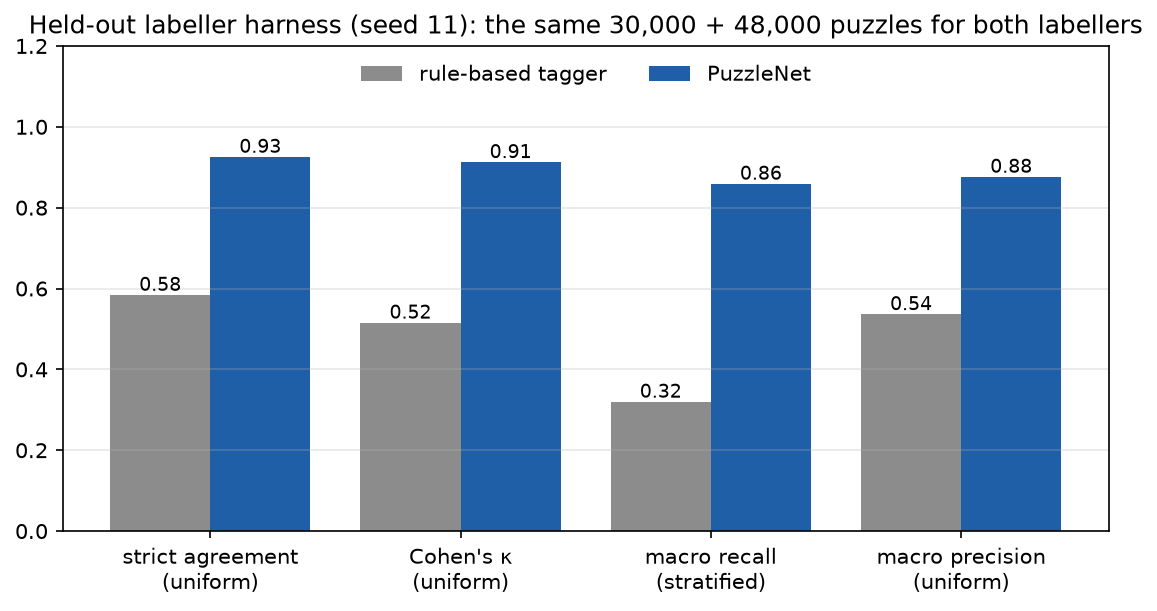
\includegraphics[width=\linewidth]{figures/nn_harness_comparison.png}
\caption{Both labellers on the held-out harness. The samples are the same puzzles that Section~\ref{sec:labeller-results} used, and neither labeller saw them during development.}\label{fig:nn-harness}
\end{figure}

The gain is largest where the rules were weakest. Macro recall nearly triples, because the tagger's
failures were structural rather than a matter of tuning: five of the 24 categories (Attraction,
Interference, Clearance, Zugzwang and X-Ray Attack) could never be emitted at all, since no
hand-written test existed for them, so their recall was zero by construction. PuzzleNet emits every
category, and learns the five missing ones from examples alone. Its remaining confusions are mostly
with the residual class \emph{General}, in both directions (for example 82 pins called General and 75
Generals called Pin): those are puzzles whose Lichess tags name no motif, where the boundary is
genuinely soft.

\begin{table}[H]
\centering
\small
\caption{Per-category recall on the stratified harness sample (2{,}000 puzzles per category where the
database has that many). The five categories in the upper block have no hand-written test at all, so
the rule-based tagger can never emit them; PuzzleNet learns them from examples.}\label{tab:nn-perclass}
\begin{tabularx}{\linewidth}{Xcccc}
\toprule
& \multicolumn{2}{c}{\textbf{Recall}} & \multicolumn{2}{c}{\textbf{Precision}} \\
\cmidrule(lr){2-3}\cmidrule(lr){4-5}
\textbf{Category} & Rules & PuzzleNet & Rules & PuzzleNet \\
\midrule
Attraction        & 0.000 & 0.869 & --- & 0.840 \\
Interference      & 0.000 & 0.714 & --- & 0.815 \\
Clearance         & 0.000 & 0.413 & --- & 0.590 \\
Zugzwang          & 0.000 & 0.618 & --- & 0.774 \\
X-Ray Attack      & 0.000 & 0.648 & --- & 0.909 \\
\midrule
En Passant        & 0.331 & 0.929 & 0.78 & 0.895 \\
Pin               & 0.227 & 0.798 & 0.43 & 0.833 \\
General           & 0.180 & 0.925 & 0.61 & 0.889 \\
Fork              & \textbf{0.956} & 0.934 & 0.61 & 0.922 \\
Mating Pattern    & 0.999 & 1.000 & 1.00 & 1.000 \\
\bottomrule
\end{tabularx}
\end{table}

Fork is the one category where the rule-based tagger has the higher recall (0.956 against 0.934), and
it shows what a rule tuned for recall costs elsewhere: its fork precision is 0.61, against 0.92 for the
network, so two of every five positions it called a fork were something else, and that misdirected
evidence went into a player's fork arm. Fourteen of the 24 categories now reach a recall of 0.9 or
better. The weakest are Clearance (0.41), Zugzwang (0.62) and X-Ray Attack (0.65) --- the motifs that
depend on what does \emph{not} happen in a line, or on long-range geometry, which a
position-and-move encoding captures least well. Lenient agreement, which accepts any category the
puzzle's own themes map to, rises from 60.9\% to 95.1\%.

\subsection{Difficulty prediction}\label{sec:nn-difficulty}

On the 174{,}754 test puzzles, the difficulty head reaches an RMSE of 268 rating points and a mean
absolute error of 205, against a rating standard deviation of 550: it explains $R^2 = 0.76$ of the
variance, with a rank correlation of $\rho = 0.88$ with the Lichess rating. The predictions are
essentially unbiased overall (mean error $-0.8$ points), but they regress to the mean at the extremes,
as any squared-error regression does: $+114$ points on puzzles rated below 1000 and $-390$ on those
above 2500.

\begin{table}[H]
\centering
\small
\caption{Difficulty prediction on the 174{,}754 test puzzles. Every baseline gets a constant
predictive standard deviation fitted on the validation split, so that the likelihoods are comparable.
The miner's formula needs an engine evaluation drop, which a Lichess puzzle does not have, so it is
evaluated with that term fixed at the median of the puzzles actually mined from users' games
(312 centipawns), which makes it a function of solution length.}\label{tab:nn-rating-baselines}
\begin{tabularx}{\linewidth}{Xcccc}
\toprule
\textbf{Difficulty model} & \textbf{RMSE} & \textbf{MAE} & \textbf{$R^2$} & \textbf{$\rho$} \\
\midrule
Constant (training mean)                          & 550 & 459 & 0.00 & --- \\
The miner's formula (what PuzzleNet replaces)     & 496 & 390 & 0.19 & 0.55 \\
Least squares on line length $\times$ mate verdict & 433 & 351 & 0.38 & 0.61 \\
Gradient-boosted trees on the hand-built features & 306 & 239 & 0.69 & 0.84 \\
\textbf{PuzzleNet}                                & \textbf{268} & \textbf{205} & \textbf{0.76} & \textbf{0.88} \\
\bottomrule
\end{tabularx}
\end{table}

The formula the system used until now explains 19\% of the variance in puzzle difficulty; the network
explains 76\%. The comparison that matters more, though, is with the gradient-boosted trees, because
they see the same hand-built tactical features and are a strong classical model on tabular data: the
network is 38 rating points better on RMSE, and on the category task it beats them by $\kappa = 0.91$
against $0.79$ with a calibration error of 0.003 against 0.123. Whatever the network is adding, it is
not only the feature engineering.

What matters more for the recommender is that the uncertainty is honest. The predictive intervals cover
what they claim to cover: 50.1\%, 81.2\% and 95.3\% of the test puzzles fall inside the nominal 50\%,
80\% and 95\% intervals. The mean content uncertainty is 240 rating points, which is the number a
mined puzzle now carries into the Bayesian update in place of the blanket 300.

\begin{table}[H]
\centering
\small
\caption{The trained network on seven textbook positions built by hand for the unit tests, none of
them from the puzzle database. $p$ is the calibrated probability of the chosen category; the rating is
the predicted difficulty with its content uncertainty.}\label{tab:nn-examples}
\begin{tabularx}{\linewidth}{Xlccl}
\toprule
\textbf{Position} & \textbf{PuzzleNet} & \textbf{$p$} & \textbf{Rating} & \textbf{Rule tagger} \\
\midrule
Back-rank mate in 1            & Mating Pattern & 1.00 & $477 \pm 83$   & Mating Pattern \\
Knight forks king and rook     & Fork           & 0.72 & $1026 \pm 196$ & Fork \\
Bishop pins knight to the king & Pin            & 0.63 & $1201 \pm 282$ & Pin \\
Rook skewers king, wins queen  & Skewer         & 1.00 & $696 \pm 58$   & Skewer \\
Pawn promotes                  & Promotion      & 0.98 & $857 \pm 162$  & Promotion \\
En passant capture             & En Passant     & 1.00 & $1137 \pm 194$ & En Passant \\
Rook ladder, mate in 2         & Mating Pattern & 1.00 & $1339 \pm 155$ & Mating Pattern \\
\bottomrule
\end{tabularx}
\end{table}

Both labellers agree on all seven, which is the expected result: these are the clean cases the rules
were written for. The interesting column is the difficulty. The network has never seen these
positions, yet it rates the mate in one at 477 with a tight interval and the two-move rook ladder at
1339, and it is least sure about the pin ($\pm 282$), which is the position whose difficulty depends
most on what the defender can try next.

\begin{figure}[H]
\centering
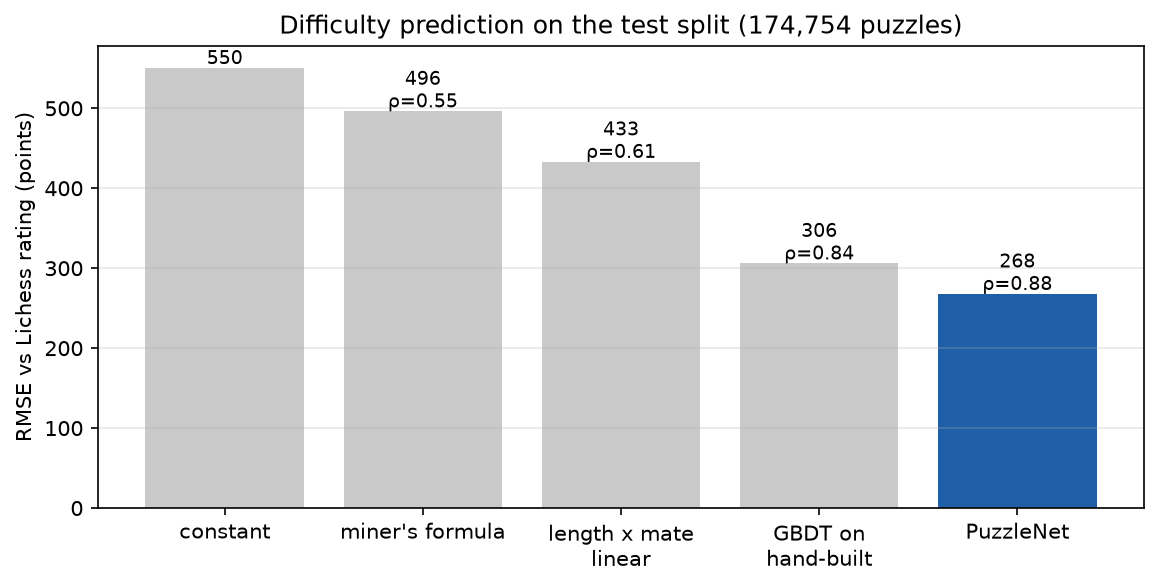
\includegraphics[width=\linewidth]{figures/nn_rating_baselines.png}
\caption{Difficulty prediction on the test split against the non-neural baselines: a constant, the miner's fixed formula, a least-squares fit on line length and the mate verdict, and gradient-boosted trees on the hand-built features. $\rho$ is the rank correlation with the Lichess rating.}\label{fig:nn-rating}
\end{figure}

\subsection{Themes and calibration}

The auxiliary theme head reaches a micro-averaged $F_1$ of 0.913 and a mean average precision of 0.817
over the 66 Lichess themes with enough positives to score. The category head is already well calibrated
before any correction (expected calibration error 0.0055) and essentially perfectly calibrated after
temperature scaling with $T = 1.08$ (0.0026). The variance scale fitted for the difficulty head is
1.05, that is, the learned variances needed almost no correction. Good calibration is not a
presentational detail here: the probabilities are consumed by the recommender, so a model that is
confidently wrong would corrupt a player's profile.

\subsection{Labelling engine lines, which is what the application actually does}\label{sec:nn-deployment}

Every number so far comes from puzzle solution lines. In the application the labeller sees something
else: Stockfish's principal variation from a critical position in a real game, cut to a fixed number
of plies. A puzzle solution stops when the tactic is complete; an engine line runs on into the won
position that follows. To measure that shift, 2{,}000 held-out harness puzzles were re-analysed with
the analyzer's own settings, and both labellers were scored on the engine line and on the solution
line of the same puzzles.

\begin{table}[H]
\centering
\small
\caption{Agreement with the Lichess category on 2{,}000 held-out puzzles, by the line the labeller is
shown. The engine's first move is the puzzle's first solution move in 99.3\% of these positions, so
the difference is about the line, not about the engine finding something else.}\label{tab:nn-engine}
\begin{tabularx}{\linewidth}{Xcc}
\toprule
\textbf{Line shown to the labeller} & \textbf{Strict agreement} & \textbf{$\kappa$} \\
\midrule
Rule-based tagger, puzzle solution        & 56.9\% & 0.504 \\
Rule-based tagger, engine line (7 plies)  & 55.5\% & 0.489 \\
\midrule
PuzzleNet, puzzle solution                & 91.9\% & 0.905 \\
PuzzleNet, engine line (1 ply)            & 66.4\% & 0.602 \\
PuzzleNet, engine line (3 plies)          & 80.3\% & 0.769 \\
\textbf{PuzzleNet, engine line (5 plies)} & \textbf{80.9\%} & \textbf{0.777} \\
PuzzleNet, engine line (7 plies)          & 76.5\% & 0.726 \\
\bottomrule
\end{tabularx}
\end{table}

\begin{honest}[Honest status: the network loses a third of its advantage in deployment]
PuzzleNet was trained on solution lines, so the engine line costs it a great deal: $\kappa$ falls from
0.91 to 0.78. The rule-based tagger barely moves (0.50 to 0.49), because it restricts which motifs may
be claimed at which depth and so ignores most of the continuation anyway. The deployed advantage is
therefore $\kappa = 0.78$ against $0.49$, not $0.91$ against $0.52$. It is still a large advantage,
and it is the honest one to quote for game analysis.
\end{honest}

The table also fixes a parameter. Agreement peaks when the network is shown five plies, and drops by
0.05 of $\kappa$ at seven, which is what the analyzer previously passed to the tagger. The deployed
system now gives the network the first five plies (\code{labeller.NEURAL\_PV\_PLIES}) and the
rule-based tagger the full line it was validated on. That is a measured choice, not a guess.

\subsection{What the network is actually learning: ablations}\label{sec:nn-ablations}

Every ablation trains on the same one-million-puzzle subset with the same schedule and is scored on
the same test split, so the rows differ only in what is named. The table is generated from
\code{eval/neural/puzzlenet\_evaluation.json} by \code{dissertation/build\_ablation\_table.py}, so it
cannot drift from the experiments.

\begin{table}[H]
\centering
\small
\caption{Ablations (1M training puzzles each) and the data-scaling sweep, all on the same test
split. $\kappa$ and macro-$F_1$ are the category head; RMSE is the difficulty head in rating points; a
dash means the model has no such head. Training times are not comparable across rows: the runs
shared a loaded laptop.}\label{tab:nn-ablations}
\begin{tabularx}{\linewidth}{Xcccc}
\toprule
\textbf{Variant} & \textbf{$\kappa$} & \textbf{Macro-$F_1$} & \textbf{RMSE} & \textbf{Train (s)} \\
\midrule
Reference: 512--256 trunk, all features, all heads & 0.867 & 0.774 & 285 & 516 \\
\midrule
No hidden layers (logistic / linear regression) & 0.743 & 0.610 & 326 & 294 \\
Raw boards and moves only & 0.741 & 0.645 & 313 & 505 \\
Hand-built relations only (no boards, no moves) & 0.830 & 0.708 & 305 & 74 \\
Wider trunk: 1024--512 & 0.878 & 0.797 & 280 & 4907 \\
\midrule
Category head alone (no multi-task) & 0.870 & 0.782 & --- & 486 \\
Difficulty head alone (no multi-task) & --- & --- & 280 & 468 \\
$\beta = 0$ (plain noise-aware likelihood) & 0.860 & 0.763 & 283 & 562 \\
$\beta = 1$ (squared-error gradient for the mean) & 0.868 & 0.777 & 289 & 250 \\
\midrule
30{,}000 training puzzles & 0.722 & 0.570 & 351 & 95 \\
100{,}000 & 0.780 & 0.654 & 333 & 127 \\
300{,}000 & 0.823 & 0.708 & 297 & 122 \\
1{,}000{,}000 & 0.867 & 0.774 & 285 & 516 \\
\textbf{5{,}526{,}626 (the production model)} & \textbf{0.914} & \textbf{0.861} & \textbf{268} & \textbf{2478} \\
\bottomrule
\end{tabularx}
\end{table}

\begin{finding}[Representation and data, not capacity]
The hand-built tactical relations carry most of the signal: on their own, with no boards and no move
blocks at all, they reach $\kappa = 0.830$ against $0.867$ for the full input. The raw boards and
moves on their own reach $0.741$. Each still adds something the other lacks --- the relations add
$0.126$ to the raw input, the raw input adds $0.037$ to the relations --- but a reader should not
conclude that the network has learned chess from squares. Depth matters about as much as the
relations: with no hidden layers, on the same features, $\kappa$ falls to $0.743$. Capacity is the
cheapest thing to buy and the least useful: four times the trunk buys $0.011$, while 5.5 times the
data buys $0.047$ and the curve has not flattened.
\end{finding}

\begin{figure}[H]
\centering
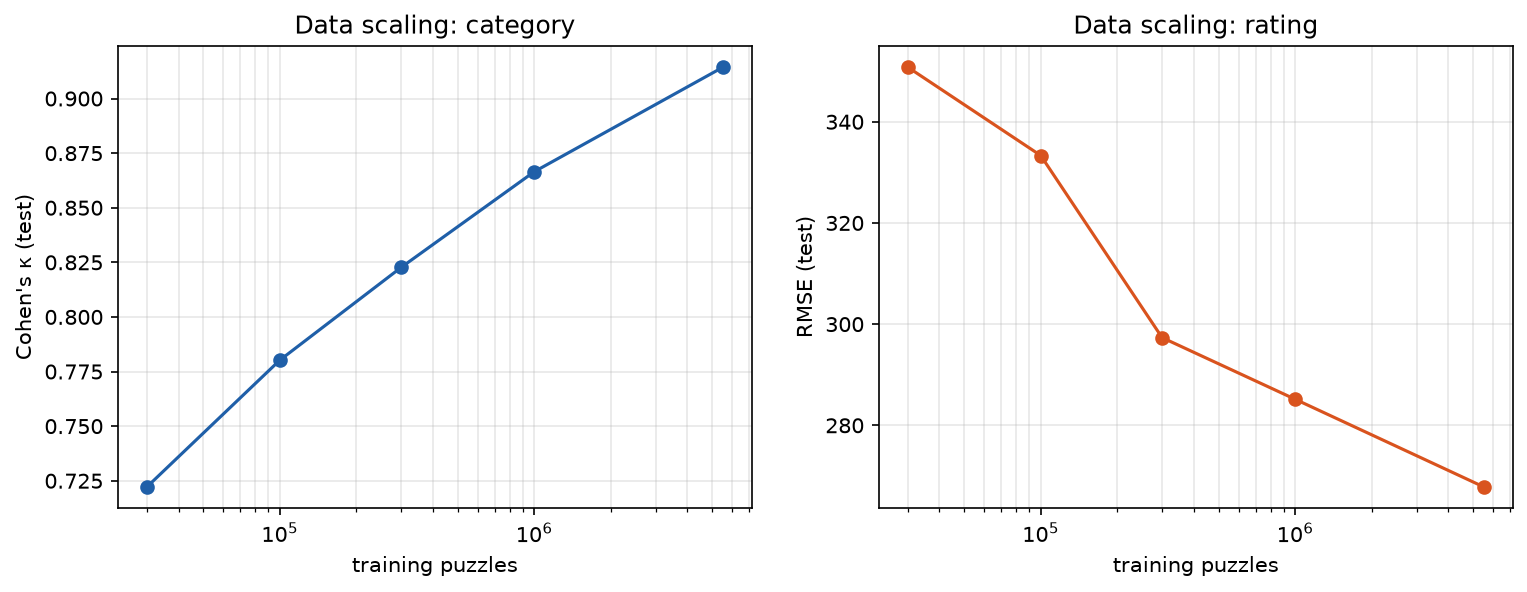
\includegraphics[width=\linewidth]{figures/nn_data_scaling.png}
\caption{Data scaling. Both heads keep improving to the full 5.5M puzzles; the curve has not flattened, so the model is limited by data rather than by capacity.}\label{fig:nn-scaling}
\end{figure}

Two results are negative and worth stating plainly. First, \textbf{multi-task learning does not help
either task here}: the category head alone reaches $\kappa = 0.870$ against $0.867$ when it shares a
trunk with themes and difficulty, and the difficulty head alone reaches RMSE 280 against 285. The
shared trunk costs a little on each task; what it buys is one model, one encoding pass and one file
instead of two, which is why the deployed model keeps it. Second, \textbf{the $\beta$-NLL correction
is not doing much work}. Plain noise-aware likelihood ($\beta = 0$) gives the best RMSE of the three
(283 against 285 at $\beta = 0.5$ and 289 at $\beta = 1$), and the differences are small either
way. The pathology that motivates
$\beta$-NLL~\cite{seitzer2022pitfalls} is that a learned variance can silence hard examples; here the
dominant part of the variance is the puzzle's \emph{known} rating deviation, and down-weighting a
noisily labelled puzzle is exactly the right thing to do, so the correction has little left to fix. On
another dataset without known label noise the argument for it would be stronger.


\subsection{Downstream: does better labelling help the recommender?}\label{sec:nn-downstream}

A labeller is only worth what it changes. Three downstream tests follow, one simulated and two on real
data, and they do not all point the same way.

\paragraph{Simulation: the label-quality bottleneck closes.} Experiment E3
(Section~\ref{sec:ablations}) measured how much early weak-category targeting depends on label
quality, by drawing each observed label from the labeller's measured $P(\text{predicted} \mid
\text{true})$. Rerunning it with PuzzleNet's confusion matrix, on the same 200 seeds so that every
comparison is paired:

\begin{table}[H]
\centering
\small
\caption{Weak-category targeting over the first 30 puzzles, by the source of the game evidence
(200 paired runs, $T = 60$).}\label{tab:nn-labelsim}
\begin{tabularx}{\linewidth}{Xcc}
\toprule
\textbf{Label source} & \textbf{Beta-TS} & \textbf{IRT-TS} \\
\midrule
No game evidence              & 0.148 & 0.151 \\
Rule-based tagger             & 0.189 & 0.226 \\
\textbf{PuzzleNet}            & \textbf{0.245} & \textbf{0.306} \\
Perfect labels                & 0.239 & 0.321 \\
\bottomrule
\end{tabularx}
\end{table}

\begin{finding}[PuzzleNet labels are statistically indistinguishable from perfect ones]
For the IRT policy, PuzzleNet beats the rule-based tagger by $+0.080$ targeting
(95\% CI $+0.055$ to $+0.105$, $p = 7 \times 10^{-10}$, $d_z = 0.46$), and the remaining gap to
\emph{perfect} labels is $+0.015$ and not significant ($p = 0.31$). It closes 84\% of the
rules-to-perfect gap for IRT-TS and all of it for Beta-TS. Cumulative regret falls from 62.6 to 55.3,
against 53.2 with perfect labels. The bottleneck identified in E3 is, in simulation, gone.
\end{finding}

\begin{figure}[H]
\centering
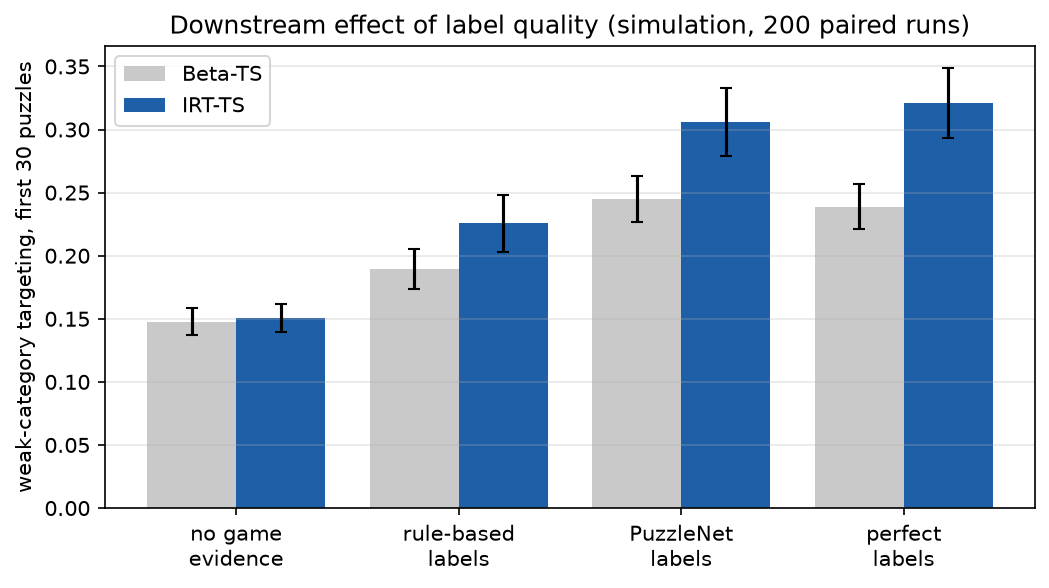
\includegraphics[width=0.8\linewidth]{figures/nn_label_simulation.png}
\caption{Downstream effect of label quality on early weak-category targeting (200 paired runs). PuzzleNet's labels are not statistically distinguishable from perfect ones.}\label{fig:nn-labelsim}
\end{figure}

\paragraph{Real players: the labels change, the diagnosis does not.} The 300-player cohort was
relabelled. Every one of the 40{,}067 critical positions was re-analysed with Stockfish at the
analyzer's own settings, and the resulting engine lines were labelled twice, once by each labeller, so
that the two versions of the cohort differ only in the labeller. Re-running the rule-based tagger on
the fresh engine lines reproduces its stored label 94.1\% of the time, which says the pipeline is
stable; the two labellers, however, agree with each other on only 37\% of real game positions. They
disagree about what players face:

\begin{table}[H]
\centering
\small
\caption{What the two labellers say the 40{,}067 critical positions of 300 real players
are.}\label{tab:nn-cohort-share}
\begin{tabularx}{\linewidth}{Xcc}
\toprule
\textbf{Category} & \textbf{Rule-based} & \textbf{PuzzleNet} \\
\midrule
Quiet Move        & 35\% & 12\% \\
General (no motif) & 11\% & 32\% \\
Endgame           & $<$1\% & 14\% \\
Fork              & 12\% & 5\% \\
Hanging Piece     & 9\% & 9\% \\
\bottomrule
\end{tabularx}
\end{table}

Given that the two labellers score $\kappa = 0.78$ and $0.49$ against an independent reference on
engine lines, the network's picture is the more credible: most critical positions in real games carry
no nameable motif, and a large share are endgame technique, while the rule-based tagger was calling a
third of everything a quiet move. That matters beyond this experiment, because the population category
norms shipped in the application (Section~\ref{sec:player-model}) were fitted on the rule-based
labels.

What does \emph{not} change is the conclusion of Section~\ref{sec:cohort-results}. With PuzzleNet
labels, split-half reliability of a player's per-category hit rates stays at zero (mean $|r| = 0.09$
across the categories with enough support, against $0.15$ before; the noise-corrected between-player
standard deviation is 0.0 under both labellings), and the ranking of the weakness models is unchanged.

\begin{finding}[Label noise was not the reason weaknesses looked like noise]
Tripling macro recall and nearly doubling $\kappa$ leaves per-category reliability at zero. The
earlier negative result therefore survives its most obvious challenge: it is not an artefact of a
crude labeller. From about 40 games, a player's per-category hit rates carry no stable
person-specific signal, whoever does the labelling, so personal weakness has to be learned online from
puzzle attempts rather than read off past games.
\end{finding}

\paragraph{Real logs: the difficulty estimate does not transfer to mined puzzles.} The third test is
the prequential replay of the application's own 123 attempts. Replacing the miner's formula with
PuzzleNet's difficulty makes the calibration \emph{worse}: log loss rises from 0.599 to 0.754.

The reason is visible in the numbers. For the 44 mined puzzles in the logs, PuzzleNet predicts a
difficulty 493 rating points higher on average than the formula (1611 against 1118), yet players solve
86.7\% of mined puzzles, against 80.0\% of Lichess pool puzzles. A mined puzzle is a position from the
player's \emph{own} game, which they have already seen at the board; it is easier for its owner than
its content suggests, and no model trained on Lichess ratings can know that. The formula's low ratings
were arbitrary, but they happened to sit closer to the truth for this population.

\begin{honest}[Honest status: the difficulty head is not used to serve mined puzzles]
The application records PuzzleNet's difficulty and uncertainty on every mined puzzle, but serves the
formula's rating unless \code{MINED\_RATING=puzzlenet} is set. Fitting the offset that would correct
the transfer needs data: a single scalar fitted on these 123 attempts runs to the edge of its range
(1181 points), which is fitting the 84.6\% base rate rather than the difficulty. The honest position
is that the difficulty head is well calibrated where it was validated --- Lichess puzzles, where its
intervals cover what they claim --- and unvalidated where the system would use it. The uncertainty it
reports is used: it is what a mined puzzle carries into the Bayesian update once the offset is known.
\end{honest}


\begin{figure}[H]
\centering
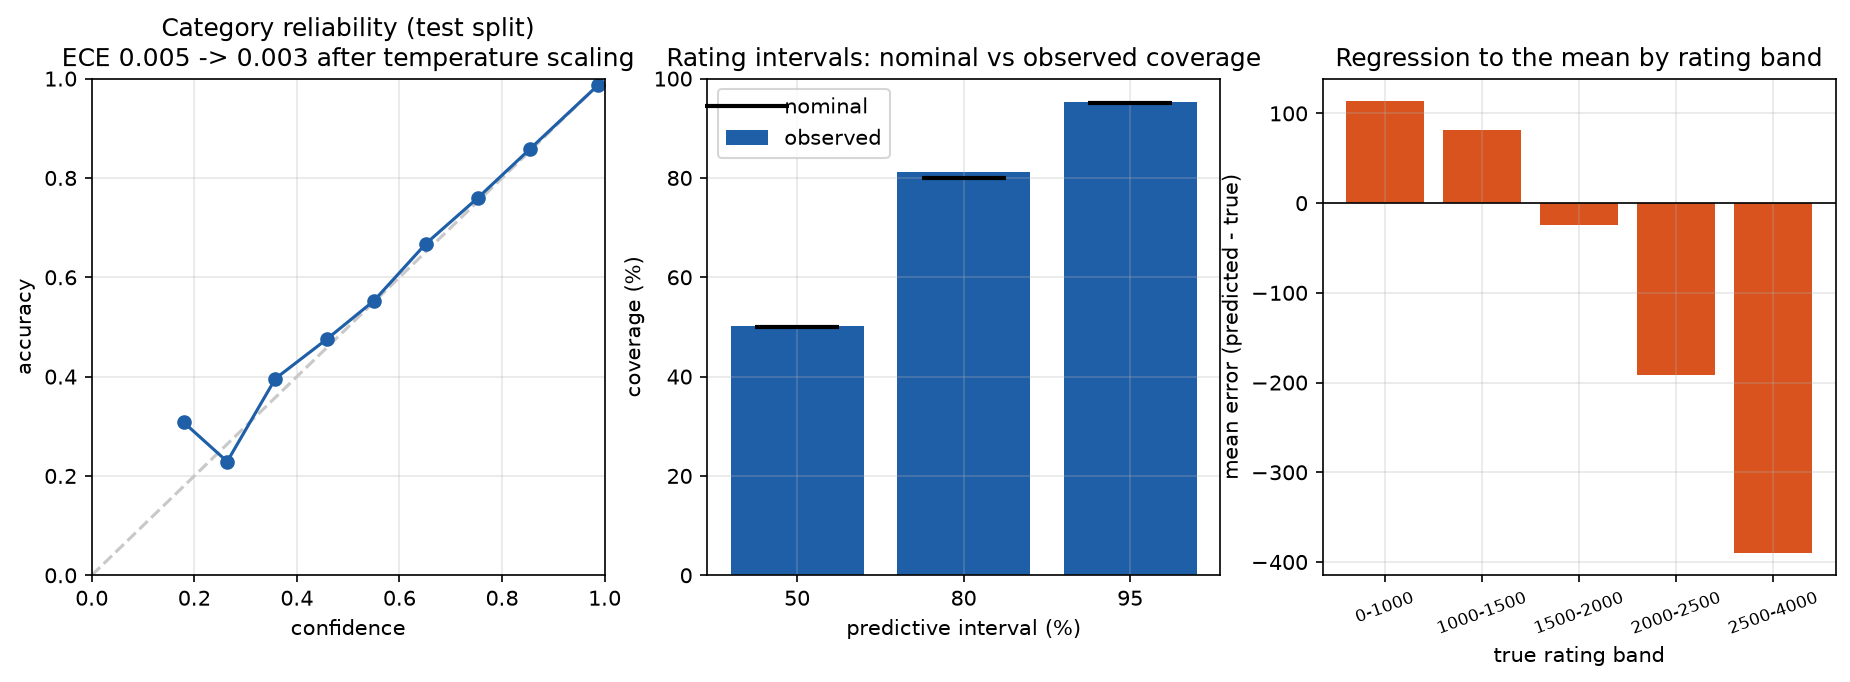
\includegraphics[width=\linewidth]{figures/nn_calibration.png}
\caption{Calibration on the test split. Left: category confidence against accuracy. Middle: how often the predicted difficulty intervals contain the Lichess rating, against what they claim. Right: the regression to the mean that a squared-error fit produces at the extremes.}\label{fig:nn-calibration}
\end{figure}


\subsection{Labelling engine lines, which is what the application actually does}\label{sec:nn-deployment}

Every number so far comes from puzzle solution lines. In the application the labeller sees something
else: Stockfish's principal variation from a critical position in a real game, cut to a fixed number
of plies. A puzzle solution stops when the tactic is complete; an engine line runs on into the won
position that follows. To measure that shift, 2{,}000 held-out harness puzzles were re-analysed with
the analyzer's own settings, and both labellers were scored on the engine line and on the solution
line of the same puzzles.

\begin{table}[H]
\centering
\small
\caption{Agreement with the Lichess category on 2{,}000 held-out puzzles, by the line the labeller is
shown. The engine's first move is the puzzle's first solution move in 99.3\% of these positions, so
the difference is about the line, not about the engine finding something else.}\label{tab:nn-engine}
\begin{tabularx}{\linewidth}{Xcc}
\toprule
\textbf{Line shown to the labeller} & \textbf{Strict agreement} & \textbf{$\kappa$} \\
\midrule
Rule-based tagger, puzzle solution        & 56.9\% & 0.504 \\
Rule-based tagger, engine line (7 plies)  & 55.5\% & 0.489 \\
\midrule
PuzzleNet, puzzle solution                & 91.9\% & 0.905 \\
PuzzleNet, engine line (1 ply)            & 66.4\% & 0.602 \\
PuzzleNet, engine line (3 plies)          & 80.3\% & 0.769 \\
\textbf{PuzzleNet, engine line (5 plies)} & \textbf{80.9\%} & \textbf{0.777} \\
PuzzleNet, engine line (7 plies)          & 76.5\% & 0.726 \\
\bottomrule
\end{tabularx}
\end{table}

\begin{honest}[Honest status: the network loses a third of its advantage in deployment]
PuzzleNet was trained on solution lines, so the engine line costs it a great deal: $\kappa$ falls from
0.91 to 0.78. The rule-based tagger barely moves (0.50 to 0.49), because it restricts which motifs may
be claimed at which depth and so ignores most of the continuation anyway. The deployed advantage is
therefore $\kappa = 0.78$ against $0.49$, not $0.91$ against $0.52$. It is still a large advantage,
and it is the honest one to quote for game analysis.
\end{honest}

The table also fixes a parameter. Agreement peaks when the network is shown five plies, and drops by
0.05 of $\kappa$ at seven, which is what the analyzer previously passed to the tagger. The deployed
system now gives the network the first five plies (\code{labeller.NEURAL\_PV\_PLIES}) and the
rule-based tagger the full line it was validated on. That is a measured choice, not a guess.

\subsection{What the network is actually learning: ablations}\label{sec:nn-ablations}

Every ablation trains on the same one-million-puzzle subset with the same schedule and is scored on
the same test split, so the rows differ only in what is named. The table is generated from
\code{eval/neural/puzzlenet\_evaluation.json} by \code{dissertation/build\_ablation\_table.py}, so it
cannot drift from the experiments.

\begin{table}[H]
\centering
\small
\caption{Ablations (1M training puzzles each) and the data-scaling sweep, all on the same test
split. $\kappa$ and macro-$F_1$ are the category head; RMSE is the difficulty head in rating points; a
dash means the model has no such head. Training times are not comparable across rows: the runs
shared a loaded laptop.}\label{tab:nn-ablations}
\begin{tabularx}{\linewidth}{Xcccc}
\toprule
\textbf{Variant} & \textbf{$\kappa$} & \textbf{Macro-$F_1$} & \textbf{RMSE} & \textbf{Train (s)} \\
\midrule
Reference: 512--256 trunk, all features, all heads & 0.867 & 0.774 & 285 & 516 \\
\midrule
No hidden layers (logistic / linear regression) & 0.743 & 0.610 & 326 & 294 \\
Raw boards and moves only & 0.741 & 0.645 & 313 & 505 \\
Hand-built relations only (no boards, no moves) & 0.830 & 0.708 & 305 & 74 \\
Wider trunk: 1024--512 & 0.878 & 0.797 & 280 & 4907 \\
\midrule
Category head alone (no multi-task) & 0.870 & 0.782 & --- & 486 \\
Difficulty head alone (no multi-task) & --- & --- & 280 & 468 \\
$\beta = 0$ (plain noise-aware likelihood) & 0.860 & 0.763 & 283 & 562 \\
$\beta = 1$ (squared-error gradient for the mean) & 0.868 & 0.777 & 289 & 250 \\
\midrule
30{,}000 training puzzles & 0.722 & 0.570 & 351 & 95 \\
100{,}000 & 0.780 & 0.654 & 333 & 127 \\
300{,}000 & 0.823 & 0.708 & 297 & 122 \\
1{,}000{,}000 & 0.867 & 0.774 & 285 & 516 \\
\textbf{5{,}526{,}626 (the production model)} & \textbf{0.914} & \textbf{0.861} & \textbf{268} & \textbf{2478} \\
\bottomrule
\end{tabularx}
\end{table}

\begin{finding}[Representation and data, not capacity]
The hand-built tactical relations carry most of the signal: on their own, with no boards and no move
blocks at all, they reach $\kappa = 0.830$ against $0.867$ for the full input. The raw boards and
moves on their own reach $0.741$. Each still adds something the other lacks --- the relations add
$0.126$ to the raw input, the raw input adds $0.037$ to the relations --- but a reader should not
conclude that the network has learned chess from squares. Depth matters about as much as the
relations: with no hidden layers, on the same features, $\kappa$ falls to $0.743$. Capacity is the
cheapest thing to buy and the least useful: four times the trunk buys $0.011$, while 5.5 times the
data buys $0.047$ and the curve has not flattened.
\end{finding}

\begin{figure}[H]
\centering
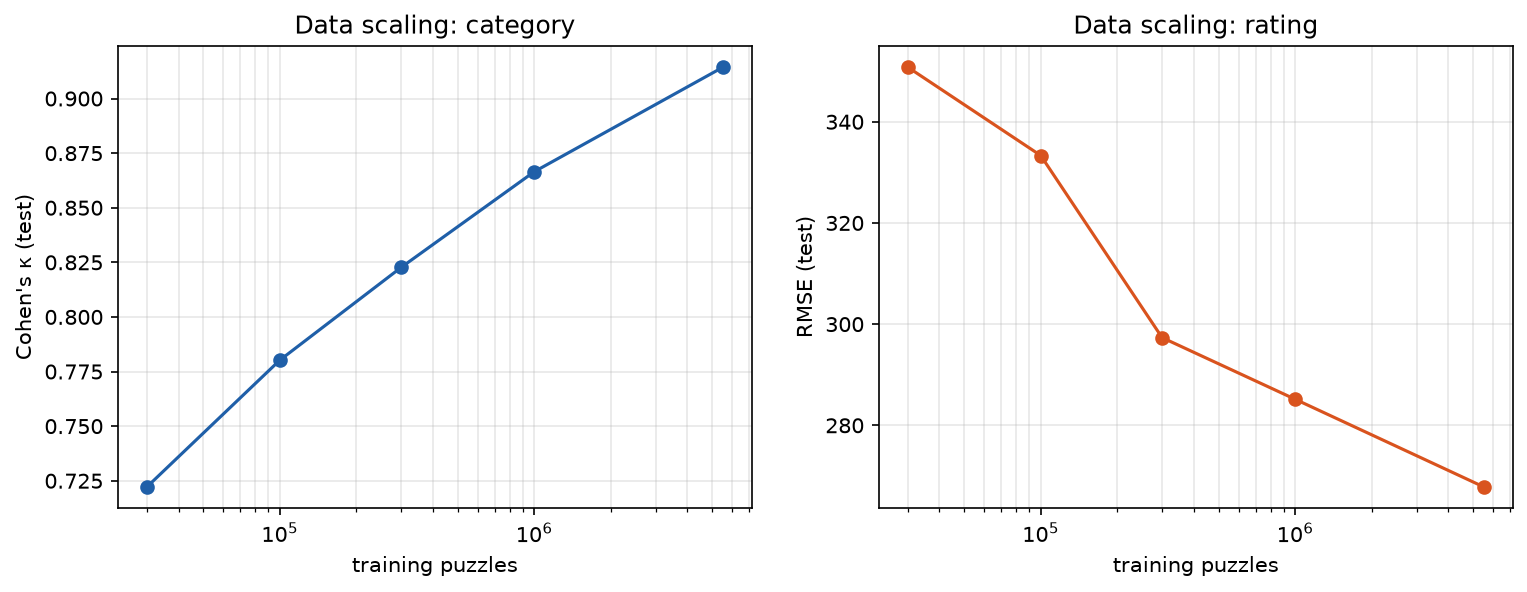
\includegraphics[width=\linewidth]{figures/nn_data_scaling.png}
\caption{Data scaling. Both heads keep improving to the full 5.5M puzzles; the curve has not flattened, so the model is limited by data rather than by capacity.}\label{fig:nn-scaling}
\end{figure}

Two results are negative and worth stating plainly. First, \textbf{multi-task learning does not help
either task here}: the category head alone reaches $\kappa = 0.870$ against $0.867$ when it shares a
trunk with themes and difficulty, and the difficulty head alone reaches RMSE 280 against 285. The
shared trunk costs a little on each task; what it buys is one model, one encoding pass and one file
instead of two, which is why the deployed model keeps it. Second, \textbf{the $\beta$-NLL correction
is not doing much work}. Plain noise-aware likelihood ($\beta = 0$) gives the best RMSE of the three
(283 against 285 at $\beta = 0.5$ and 289 at $\beta = 1$), and the differences are small either
way. The pathology that motivates
$\beta$-NLL~\cite{seitzer2022pitfalls} is that a learned variance can silence hard examples; here the
dominant part of the variance is the puzzle's \emph{known} rating deviation, and down-weighting a
noisily labelled puzzle is exactly the right thing to do, so the correction has little left to fix. On
another dataset without known label noise the argument for it would be stronger.


\subsection{Downstream: does better labelling help the recommender?}\label{sec:nn-downstream}

A labeller is only worth what it changes. Three downstream tests follow, one simulated and two on real
data, and they do not all point the same way.

\paragraph{Simulation: the label-quality bottleneck closes.} Experiment E3
(Section~\ref{sec:ablations}) measured how much early weak-category targeting depends on label
quality, by drawing each observed label from the labeller's measured $P(\text{predicted} \mid
\text{true})$. Rerunning it with PuzzleNet's confusion matrix, on the same 200 seeds so that every
comparison is paired:

\begin{table}[H]
\centering
\small
\caption{Weak-category targeting over the first 30 puzzles, by the source of the game evidence
(200 paired runs, $T = 60$).}\label{tab:nn-labelsim}
\begin{tabularx}{\linewidth}{Xcc}
\toprule
\textbf{Label source} & \textbf{Beta-TS} & \textbf{IRT-TS} \\
\midrule
No game evidence              & 0.148 & 0.151 \\
Rule-based tagger             & 0.189 & 0.226 \\
\textbf{PuzzleNet}            & \textbf{0.245} & \textbf{0.306} \\
Perfect labels                & 0.239 & 0.321 \\
\bottomrule
\end{tabularx}
\end{table}

\begin{finding}[PuzzleNet labels are statistically indistinguishable from perfect ones]
For the IRT policy, PuzzleNet beats the rule-based tagger by $+0.080$ targeting
(95\% CI $+0.055$ to $+0.105$, $p = 7 \times 10^{-10}$, $d_z = 0.46$), and the remaining gap to
\emph{perfect} labels is $+0.015$ and not significant ($p = 0.31$). It closes 84\% of the
rules-to-perfect gap for IRT-TS and all of it for Beta-TS. Cumulative regret falls from 62.6 to 55.3,
against 53.2 with perfect labels. The bottleneck identified in E3 is, in simulation, gone.
\end{finding}

\begin{figure}[H]
\centering
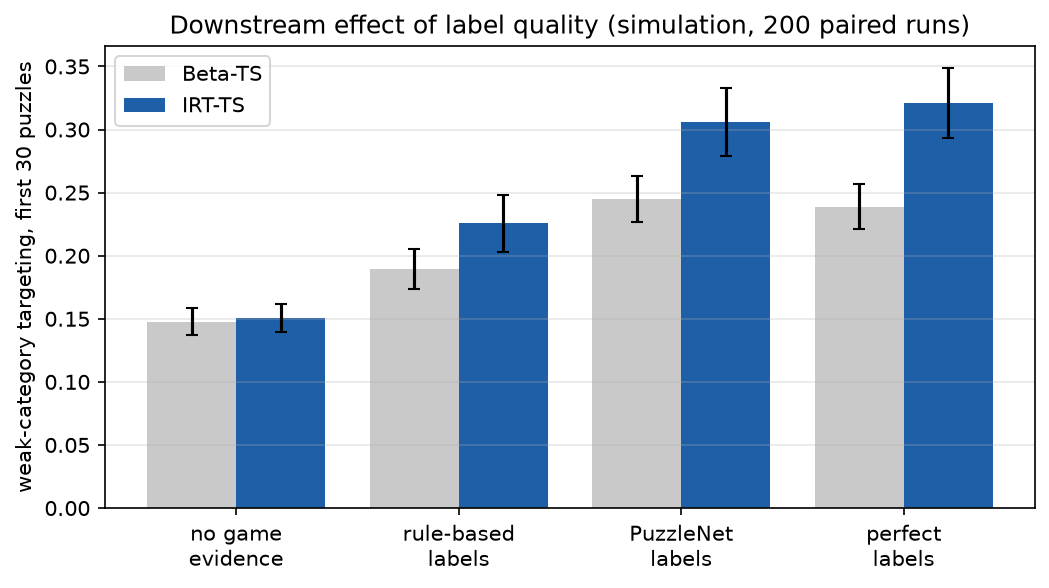
\includegraphics[width=0.8\linewidth]{figures/nn_label_simulation.png}
\caption{Downstream effect of label quality on early weak-category targeting (200 paired runs). PuzzleNet's labels are not statistically distinguishable from perfect ones.}\label{fig:nn-labelsim}
\end{figure}

\paragraph{Real players: the labels change, the diagnosis does not.} The 300-player cohort was
relabelled. Every one of the 40{,}067 critical positions was re-analysed with Stockfish at the
analyzer's own settings, and the resulting engine lines were labelled twice, once by each labeller, so
that the two versions of the cohort differ only in the labeller. Re-running the rule-based tagger on
the fresh engine lines reproduces its stored label 94.1\% of the time, which says the pipeline is
stable; the two labellers, however, agree with each other on only 37\% of real game positions. They
disagree about what players face:

\begin{table}[H]
\centering
\small
\caption{What the two labellers say the 40{,}067 critical positions of 300 real players
are.}\label{tab:nn-cohort-share}
\begin{tabularx}{\linewidth}{Xcc}
\toprule
\textbf{Category} & \textbf{Rule-based} & \textbf{PuzzleNet} \\
\midrule
Quiet Move        & 35\% & 12\% \\
General (no motif) & 11\% & 32\% \\
Endgame           & $<$1\% & 14\% \\
Fork              & 12\% & 5\% \\
Hanging Piece     & 9\% & 9\% \\
\bottomrule
\end{tabularx}
\end{table}

Given that the two labellers score $\kappa = 0.78$ and $0.49$ against an independent reference on
engine lines, the network's picture is the more credible: most critical positions in real games carry
no nameable motif, and a large share are endgame technique, while the rule-based tagger was calling a
third of everything a quiet move. That matters beyond this experiment, because the population category
norms shipped in the application (Section~\ref{sec:player-model}) were fitted on the rule-based
labels.

What does \emph{not} change is the conclusion of Section~\ref{sec:cohort-results}. With PuzzleNet
labels, split-half reliability of a player's per-category hit rates stays at zero (mean $|r| = 0.09$
across the categories with enough support, against $0.15$ before; the noise-corrected between-player
standard deviation is 0.0 under both labellings), and the ranking of the weakness models is unchanged.

\begin{finding}[Label noise was not the reason weaknesses looked like noise]
Tripling macro recall and nearly doubling $\kappa$ leaves per-category reliability at zero. The
earlier negative result therefore survives its most obvious challenge: it is not an artefact of a
crude labeller. From about 40 games, a player's per-category hit rates carry no stable
person-specific signal, whoever does the labelling, so personal weakness has to be learned online from
puzzle attempts rather than read off past games.
\end{finding}

\paragraph{Real logs: the difficulty estimate does not transfer to mined puzzles.} The third test is
the prequential replay of the application's own 123 attempts. Replacing the miner's formula with
PuzzleNet's difficulty makes the calibration \emph{worse}: log loss rises from 0.599 to 0.754.

The reason is visible in the numbers. For the 44 mined puzzles in the logs, PuzzleNet predicts a
difficulty 493 rating points higher on average than the formula (1611 against 1118), yet players solve
86.7\% of mined puzzles, against 80.0\% of Lichess pool puzzles. A mined puzzle is a position from the
player's \emph{own} game, which they have already seen at the board; it is easier for its owner than
its content suggests, and no model trained on Lichess ratings can know that. The formula's low ratings
were arbitrary, but they happened to sit closer to the truth for this population.

\begin{honest}[Honest status: the difficulty head is not used to serve mined puzzles]
The application records PuzzleNet's difficulty and uncertainty on every mined puzzle, but serves the
formula's rating unless \code{MINED\_RATING=puzzlenet} is set. Fitting the offset that would correct
the transfer needs data: a single scalar fitted on these 123 attempts runs to the edge of its range
(1181 points), which is fitting the 84.6\% base rate rather than the difficulty. The honest position
is that the difficulty head is well calibrated where it was validated --- Lichess puzzles, where its
intervals cover what they claim --- and unvalidated where the system would use it. The uncertainty it
reports is used: it is what a mined puzzle carries into the Bayesian update once the offset is known.
\end{honest}

